%Num-Projekt1, Amanda ? , Christoph Mayer

\documentclass[a4paper,11pt,bibliography=totoc,listof=totoc,headinclude=true,cleardoublepage=empty,oneside]{scrbook}
% Option "oneside" für einseitigen Druck. Weglassen, falls die Arbeit doppelseitig gedruckt wird
\usepackage{graphicx} 
\usepackage[english,ngerman]{babel}
\usepackage[utf8]{inputenc}
%\usepackage{fullpage}
\usepackage{ifthen}
\usepackage{color}
\usepackage{amsmath,amsthm,amssymb,amsfonts}
\usepackage{graphicx}
\usepackage{amsmath}
\usepackage{mathtools}
\usepackage{tikz}
% links in pdf
\usepackage[unicode,colorlinks=true,pagebackref=false]{hyperref}
\usepackage{listings}
%\usepackage{maplestd2e}
% Zum Druck verwende schwarze Links!
%\usepackage[unicode,colorlinks=true,linkcolor=black,citecolor=black,urlcolor=black,pagebackref=false]{hyperref} 
% colorlinks=false umrahmt Links statt einzufaerben, 

\counterwithout{figure}{chapter}


% document style
\KOMAoptions{footinclude=false} % Fusszeile wird nicht zu Satzspiegel gezaehlt
\KOMAoptions{headsepline=true} % Trennlinie zwischen Kopfzeile und Text
\KOMAoptions{DIV=12} % beeinflusst Satzspiegel
\KOMAoptions{BCOR=8mm} % Bindekorrektur
\pagestyle{headings} % mit Kopfzeilen

\recalctypearea % berechne Satzspiegel neu

\definecolor{change}{rgb}{0,.55,.55}
\definecolor{change2}{rgb}{0,0,0}
\definecolor{change3}{rgb}{0.5,0,0}

\def\revision#1{{\color{red}#1}}

\lstset{ 
	language=Matlab, 
	showstringspaces=false}

\newcommand{\code}[1]{\texttt{\color{change}#1}}
\DeclareMathOperator*{\SPAN}{span}
\DeclareMathOperator*{\conv}{conv}

%%%%%%%%%%%%%%%%%%%%%%%%%%%%%%%%%%%%%%%%%%%%%%%%%%%%%%%%%%%%%%%%%%%%%%%%%%%%%%%%%%%%%%%%%%%%%%%%%%%%%%%%%%%%%%
%%%%%%%%%%%%%%%%%%%%%%%%%%%%%%%%%%%%%%%%%%%%%%%%%%%%%%%%%%%%%%%%%%%%%%%%%%%%%%%%%%%%%%%%%%%%%%%%%%%%%%%%%%%%%%
%%%%%%%%%%%%%%%%%%%%%%%%%%%%%%%%%%%%%%%%%%%%%%%%%%%%%%%%%%%%%%%%%%%%%%%%%%%%%%%%%%%%%%%%%%%%%%%%%%%%%%%%%%%%%%
%%%%%%%%%%%%%%%%%%%%%%%%%%%%%%%%%%%%%%%%%%%%%%%%%%%%%%%%%%%%%%%%%%%%%%%%%%%%%%%%%%%%%%%%%%%%%%%%%%%%%%%%%%%%%%

\begin{document}


\pagenumbering{arabic}
\selectlanguage{ngerman}

\begin{titlepage}
	%\vspace*{-2cm}
	\begin{center}
	%	\includegraphics[width=0.45\textwidth]{TULogo.eps}
		\vskip 1cm%
		{\LARGE N~\Large U~M~E~R~I~K}
		\vskip 8mm
		{\huge\bfseries Projekt 1}
		\vskip 1cm
		
		{\Large\bfseries Name des Tutors: Johann Faschingleitner}\\[1ex]
		\vskip 0.5cm
		{\Large\bfseries Name der Autoren:}\\[1ex]
		\vskip 0.5cm
		Amanda Schöfl
		\vskip 0.5cm
		Matrikelnummer: e0271473\\[1ex]
		\vskip 0.5cm
		Christoph Mayer
		\vskip 0.5cm
		Matrikelnummer: e01425430\\[1ex]

		
	\end{center}
\end{titlepage}

\cleardoublepage
	
\chapter*{Aufgabe 3} %\chapter*{Acknowledgement}
\thispagestyle{empty}
\selectlanguage{ngerman} %\selectlanguage{english}

\subsubsection{3.1 Aufgabenstellung}
Basierend auf einer 1D Quadratur kann durch Bildung des Tensorproduktes eine 2D Quadratur erzeugt werden. Sei dazu $f:	\mathbb{R} ^2 \to \mathbb{R}$ eine auf dem Einheitsqudrat $Q:=[0,1]\times[0,1]$ integrierbare Funktion, dann gilt (mittels Fubini)
		
\begin{equation}\label{equ:integral}
\begin{array}{rccll}
	\int\limits_{\hat{Q}}f(x,y)d(x,y)&=&\int\limits_{0}^{1}\Big(\int\limits_{0}^{1}f(x,y)dx\Big)dy&=&\\
	&=&\int\limits_0^{1}\Big(\sum\limits_{i=0}^n\alpha_i f(x_i,y)\Big)dy &=&\\ 
	&=&\sum\limits_{i=0}^n \alpha_i \int\limits_0^{1} f(x_i,y)dy&=&\\
	&=&\sum\limits_{i=0}^{n} \alpha_i\Big(\sum\limits_{j=0}^{n} \alpha_j f(x_i,y_i)\Big)&=&\sum\limits_{i,j=0}^{n} \alpha_i\alpha_j f(x_i,y_j),\\
\end{array}
\end{equation}
wobei $\{\alpha_i: i=0,...n\}$ und  $\{x_i,y_j : i,j=0,...n\}$ die 1D Quadraturgewichte und -knoten sind. Somit kann man mit den bereits bekannte 1D Quadraturen auch Integrale am Einheitsquadrat numerisch berechnen. Implementieren Sie mit Hilfe des zur Verfügung gestellten Programms \textbf{gauss(n)} eine Funktion \textbf{quadInt(f,n)} die $\int_{\hat{Q}}f(x,y)d(x,y) $ berechnet. Für welche n wird ein Polynom $ p \in \prod_{2}^k:=\SPAN\{x^iy^j:0 \leq i,j\leq k \} $ exakt integriert?

\subsubsection{3.1 Durchführung}

Die folgende Implementierung der Funktion \textbf{quadInt}, hat die Inputparameter
\begin{itemize}
	\item \code{f} ein Function Handle einer Funktion mit oben beschriebenen Eigenschaften,
	\item \code{n} der Grad der Gaußquadratur.
\end{itemize} 
Sie gibt den approximierten Wert des Integrals der übergebenen Funktion auf $\hat{Q}$ zurück.
{
	\color{change}		
%\lstset{ 
%	language=Matlab, 
%	showstringspaces=false}
\lstinputlisting{quadInt.m} 
		
%		\begin{lstlisting}
%
%		\end{lstlisting}
% Was tut das??
}
Widmen wir uns jetzt noch der Frage für welche $n$ ein Polynom $ p \in \prod_{2}^k:=\SPAN\{x^iy^j:0 \leq i,j\leq k \} $ exakt integriert wird.		
Wir wissen, dass mittels 1D Quadraturen vom Grad $n$ Polynome vom Grad $2n+1$ exakt numerisch berechnet werden können. Sei die in \ref{equ:integral} vorkommende Funktion $f$ nun unser Polynom $p$. Da zunächst nach $x$ integriert wird, wirken die in $p$ vorkommenden $y$ bloß als reelle Koeffizienten. Somit kann $p$ genau dann numerisch exakt nach $x$ integriert werden, wenn das Polynom
\begin{equation*}
	x \mapsto p_y(x) := p(x,y)
\end{equation*}
für feste $y$ höchstens vom Grad $2n+1$ ist. Analoges gilt für die Integration nach $y$. Damit kann $p$ genau für $k \leq 2n+1$ exakt integriert werden.



% Da in \ref{equ:integral} lediglich die Gauß-Quadratur 2-mal hintereinander eindimensional durchgeführt wird, gilt, dass i=2n+1 und j=2n+1 die höchsten Grade sind, für welche die 2D Quadratur exakt numerisch berechnet werden kann.


\subsubsection{3.2 Aufgabenstellung}
Da zum Beispiel bei der Finite-Element-Methode eine Quadratur auf Dreiecken benötigt wird, verwendet man gerne die \textit{Duffy-Transformation} um die Quadratur auf dem Einheitsquadrat \^{Q} auf das Referenzdreieck \^{T} mit den Eckpunkten $ (0,0),(1,0)$ und $ (0,1)$ zu transformieren.
Die \textit{Duffy-Transformation} ist definiert als:

\begin{equation}\label{equ:duffy}
\Psi = \begin{cases} 
\hat{Q} \to \hat{T} \\
(s,t) \mapsto (s,(1-s)t)
\end{cases} 
\end{equation} 
\\
Implementieren Sie mithilfe der \textit{Duffy-Transformation} die Funktion \textbf{trigInt(f,n)}, sodass Sie Integrale auf \^{T} berechnen können.
\textit{Hinweis}: Verwenden Sie dazu die Substitutionsregel Satz 7.34 (Transformationssatz für Integrale) aus dem Analysis-Skript von Professor Engl.


\subsubsection{3.2 Durchführung}
\vspace{0.5cm}
\setlength{\fboxsep}{1em}
\fbox{
	\parbox{35.5em}{Transformationssatz für Integrale:
		
		Es sei $\Omega \in \mathbb{R}$ eine offene Menge und $\Phi:\Omega \to \Phi(\Omega) \in \mathbb{R}^d$ ein Diffeomorphismus. Dann ist die Funktion $f$ auf $\Phi(\Omega)$ genau dann integrierbar, wenn die Funktion $x \mapsto f(\Phi(x)) |\det(D\Phi(x))| $ auf $\Omega$ integrierbar ist.
		In diesem Fall gilt: \linebreak
	\begin{equation*}
		\int_{\Phi(\Omega)}f(y)dy = \int_{\Omega}f(\Phi(x))|\det(D\Phi(x))|dx.
	\end{equation*}
	
		Dabei ist $D\Phi(x)$ die Jacobi-Matrix und $\det(D\Phi(x))$ die Funktionaldeterminante  von $\Phi$, also $Df(\Phi)=\Big(\frac{\partial f_i}{\partial x_j}(x)\Big)_{i,j=1,...,n}$.}}
\vspace{0.5cm}
		% Funktionaldeterminante anpassen
		
In unserem Fall sei $\Omega=(0,1)\times(0,1)$. Dies entspricht der Menge $\hat{Q}$ ohne Rand, welcher jedoch eine Nullmenge bezüglich des zweidimensionalen Lebesguemaß darstellt und somit $\int_{(0,1)\times(0,1)}f(x)dx = \int_{\hat{Q}}f(x)dx$ gilt. Analog ist das Integral einer Funktion über $\hat{T}$ ident mit jenem über $\hat{T}$ ohne den Rand $\partial\hat{T}$. Für $\Phi$ wählen wir die Abbildung $\Psi$. Diese ist offenbar unendlich oft stetig differenzierbar, hat auf $\hat{T}\backslash\partial\hat{T}$ mit 
\begin{equation*} 
	\Psi^{-1} := \begin{cases} 
	\hat{T}\backslash\partial\hat{T}\ \to \hat{Q}\backslash\partial\hat{Q} \\
	(x,y) \mapsto (x,\frac{y}{(1-x)})
	\end{cases} 
\end{equation*} 
eine überall stetig differenzierbare Umkehrabbildung. $\Psi$ eingeschränkt auf $\hat{Q}\backslash\partial\hat{Q}$ ist folglich bijektiv und erfüllt damit alle Voraussetzungen für einen Diffeomorphismus. Die Funktionaldeterminante von $\Psi$ ergibt sich gemäß
		
\begin{equation*}
	\det \Psi = |\det		
	\left(
	\begin{array}{cc}
	1 & -t \\
	0 & (1-s)\\
	\end{array}
	\right)| = |(1-s)|.
\end{equation*}
Nach dem Transformationssatz gilt folglich
\begin{equation*} \label{eq1}
	\int_{\hat{T}}f(x,y)d(x,y) = \int_{\hat{Q}}f(s,(1-s)t)|(1-s)|d(t,s).
\end{equation*}
Das Rechte Integral lässt sich nun analog zur vorherigen Aufgabe berechnen. 

Die folgende Implementierung der Funktion \textbf{trigInt}, hat die Inputparameter
\begin{itemize}
	\item \code{f} ein Function Handle einer Funktion mit oben beschriebenen Eigenschaften auf dem Dreieck $\hat{T}$,
	\item \code{n} der Grad der Gaußquadratur.
\end{itemize} 
Sie gibt den approximierten Wert des Integrals der Funktion $f$ auf dem Gebiet $\hat{T}$ zurück.
		
{\color{change}
\lstset{ 
	language=Matlab, 
	showstringspaces=false}
\lstinputlisting{trigInt.m}}

\subsubsection{3.3 Aufgabenstellung}

Erweitern Sie unter Verwendung einer affinen Transformation $\Phi_T:\hat{T} \to T$ Ihre Implementierung von $\textbf{duffyInt}$, um auch Integralen auf beliebigen Dreiecken T berechnen zu können. 
Für welche n wird ein Polynom $ p \in \prod_{2}^k:=\SPAN\{x^iy^j:0 \leq i+j\leq k \} $ exakt integriert? \\

\noindent \textit{Hinweis:} Sie können die Implementation Ihrer Transformation testen, indem Sie das Integral über $f \equiv1$ numerisch berechnen und mit der analytisch bestimmten Fläche des Dreiecks T vergleichen.


\subsubsection{3.3 Durchführung}

Anstatt einer affinen Transformation von $ \Phi_{\hat{T}}:\hat{T} \to T$ verwenden wir eine affine Transformation $\Phi:\hat{Q} \mapsto T$. \\

\noindent Sei nun T ein beliebiges Dreieck mit den Eckpunkten $a=\left(\begin{array}{ccc}
				a_1 \\
				a_2\\
		\end{array}\right)$, 
$b=\left(\begin{array}{ccc}
				b_1 \\
				b_2\\
		\end{array}\right)$,
$c=\left(\begin{array}{ccc}
				c_1 \\
				c_2\\
		\end{array}\right)$.
		
\vspace{4mm}\hspace{3.6cm}
\begin{tikzpicture}
%Koordinaten für die Beschriftung 
\coordinate[label=left:$a$]  (A) at (5,0); 
\coordinate[label=right:$b$] (B) at (10,2); 
\coordinate[label=above:$c$] (C) at (6,2.5); 

\draw[-] (A) -- (B) -- (C) -- (A);
%warum funktioniert vektor nicht?
\path [->] 
(A) edge node [left]{$\vec{v}$} (C)   ;
\path[->]
(B) edge node [above]{$\vec{w}$} (C) ;  
\end{tikzpicture}
\vspace{4mm}

\noindent Die Fläche des Dreiecks ist nun genau die Konvexe Hülle der Eckpunkte. Um diese zu bilden, betrachten wir zunächst die Vektoren  

\begin{equation*}
	v=\left(
	\begin{array}{ccc}
	(1-s)a_1+ sc_1\\
	(1-s)a_2+sc_2\\
	\end{array}
	\right) \text{ und } w=\left(
	\begin{array}{ccc}
	(1-s)b_1+ sc_1\\
	(1-s)b_2+sc_2\\
	\end{array}
	\right). 
\end{equation*}

\noindent Aus einer Kombination $(1-t)v+tw$ dieser Vektoren ergibt sich nun eine Parametrisierung $\Phi$ des Dreiecks gemäß 

\begin{equation*}
	\Phi = \begin{cases} 
	\hat{Q} \to T \\
	(s,t) \mapsto \left(
	\begin{array}{ccc}
	a_1 + s(c_1-a_1)+ t(b_1-a_1) + st(a_1-b_1)\\
	a_2 + s(c_2-a_2) + t(b_2-a_2) + st(a_2-b_2)\\
	\end{array}
	\right).
	\end{cases}
\end{equation*}


\noindent Setzt man nun die Eckpunkte  aus Aufgabe 3.2 ein, also 

\begin{equation*}
	a=\left(
	\begin{array}{ccc}
	0 \\
	0\\
	\end{array}
	\right), b=\left(
	\begin{array}{ccc}
	0 \\
	1\\
	\end{array}
	\right), c=\left(
	\begin{array}{ccc}
	1\\
	0\\
	\end{array}
	\right),
\end{equation*}

\noindent ergibt sich genau die  Duffy-Transformation

\begin{equation}
	(s,t) \mapsto  \left(
	\begin{array}{ccc}
	t-st\\
	s\\
	\end{array}
	\right) = \left(
	\begin{array}{ccc}
	t(1-s)\\
	s\\
	\end{array}
	\right).
\end{equation}

Die Implementierung der Funktion erfolgt nun analog zur vorherigen Aufgabe. 
Die Funktion \textbf{duffyInt}, hat die Inputparameter
\begin{itemize}
\item \code{f} ein Function Handle einer Funktion mit oben beschriebenen Eigenschaften,
\item \code{n} der Grad der Gaußquadratur.
\item \code{$a_1,a_2$} : Koordinaten des Punktes a
\item \code{$b_1,b_2$} : Koordinaten des Punktes b
\item \code{$c_1,c_2$} : Koordinaten des Punktes c
\end{itemize} 
Sie gibt den approximierten Wert des Integrals nach der Transformation auf ein beliebiges Dreieck mit den Eckpunkten (a,b,c) zurück.

{\color{change}
\lstset{ 
language=Matlab, 
showstringspaces=false}
\lstinputlisting{duffyInt.m} }




Widmen wir uns nun noch der Frage wann ein Polynom $ p \in \prod_{2}^k:=\SPAN\{x^iy^j:0 \leq i+j\leq k \} $ exakt integriert werden kann.Da $p$ eine Linearkombination von Polynomen der Gestalt $(x,y) \mapsto x^iy^j$ ist, reicht es das Polynom $q(x,y) = x^iy^j$ zu betrachten. Unter der Transformation $\Phi$ wird $q$ zu 
\begin{equation*}
	q(\Phi(x),\Phi(y)) = (\alpha_1+s\alpha_2+t\alpha_3+st\alpha_4)^i(\beta_1+s\beta_2+t\beta_3+st\beta_4)^j.
\end{equation*}
Durch Ausmultiplizieren wird ersichtlich, dass es sich dabei um ein Polynom vom Grad $i+j$ in $s$ und $t$ handelt. Das heißt der Term mit den höchsten Potenzen von $s$ und $t$ ist von der Gestalt $cs^it^is^jt^j = cs^{(i+j)}t^{(i+j)}$ mit einer reellen Konstanten $c$. Für die Integration über $T$ wird dieser Ausdruck nun noch mit dem Betrag der Funktionaldeterminante multipliziert. Darin kommen $s$ und $t$ jeweils linear vor. Der Summand mit den höchsten Potenzen ist also von Gestalt $\tilde{c}st$ mit einer reellen Konstanten $\tilde{c}$. Insgesamt ergibt sich, für den Integranden von 
\begin{equation*}
	\int_{\hat{Q}}^{} p(\Phi(x),\Phi(y)) \det|d\Phi| d(s,t)
\end{equation*}
ein Polynom in $s$ und $t$, welches jeweils vom Grad $i+j+1$ ist. Auf Grund vorher bereits angestellter Überlegungen, wissen wir, dass dies genau für $i+j+1 \leq 2n+1$ mittels einer 2D-Quadratur vom Grad $n$ exakt numerisch integriert werden kann. Insgesamt gilt also, dass für $k \leq 2n$ eine exakte numerische Integration gegeben ist. 


\subsubsection{3.4 Aufgabenstellung} 
Erweitern Sie Ihre Implementierung von \textbf{quadInt(f,n)} zur Berechnung von Integralen auf beliebigen konvexen Vierecken $ Q=\conv{(a1,a2),(b1,b2),(c1,c2),(d1,d2)} $. Verwenden Sie dazu eine eine Transformation der Form:

\begin{equation*} 
\Psi_{\hat{Q}} = \begin{cases} 
\hat{Q} \to Q \\
(s,t) \mapsto

\left(
\begin{array}{ccc}
\alpha_1 + \alpha_{2}s + \alpha_{3}t +\alpha_{4}st \\
\beta_1+\beta_{2}s+\beta_{3}t+\beta_{4}st \\
\end{array}
\right)

\end{cases} 
\end{equation*} \\

\color{change2}
\begin{flushleft}		mit den Konstanten $\alpha_i$,$\beta_i \in \mathbb{R}$. Überlegen Sie sich, warum nicht-konvexe Vierecke unzulässig sind.\end{flushleft} 
\vspace*{3mm}

\subsubsection{3.4 Durchführung}

Sei $Q$ nun ein beliebiges konvexes Viereck mit den Eckpunkten $a=\left(\begin{array}{ccc}
a_1 \\
a_2\\
\end{array}\right)$, 
$b=\left(\begin{array}{ccc}
b_1 \\
b_2\\
\end{array}\right)$,
$c=\left(\begin{array}{ccc}
c_1 \\
c_2\\
\end{array}\right)$,
$d=\left(\begin{array}{ccc}
d_1 \\
d_2\\
\end{array}\right)$.

\hspace*{3.5cm}\begin{tikzpicture} 
%Koordinaten für die Beschriftung 
\coordinate[label=left:$a$]  (A) at (0,0); 
\coordinate[label=left:$d$] (D) at (2,3); 
\coordinate[label=above:$c$] (C) at (3.5,3.5);
\coordinate[label=right:$b$] (B) at (3.5,1); 

\draw (A) -- (B) -- (C) -- (D) -- (A);
\path [->] 
(A) edge node [left]{$\vec{v}$} (D)   
(B) edge node [right]{$\vec{w}$} (C)   
; 
\end{tikzpicture}

Die Fläche des Vierecks geht nun aus einer zu Aufgabe 3.3 analogen Konvexkombination $\vec{v}(1-t)+\vec{w}t$ aus den Vektoren $\vec{v} = a(1-s)+ds$ und $\vec{w} = b(1-s)+cs$ hervor. Aus der Tatsache, dass die Transformation aus der Angabe äquivalent zu einer Konvexkombination der Eckpunkte des Vierecks ist, geht auch hervor, dass nicht konvexe Vielecke damit nicht abgebildet werden können.


Nun ergeben sich die Konstanten $\alpha_i, \beta_i$ entweder durch das Ausmultiplizieren der obigen Konvexkombination oder dem Lösen eines Gleichungssystems, wenn man davon ausgeht dass die Eckpunkte von $\hat{Q}$ jeweils auf die Eckpunkte von $Q$ abgebildet werden. \\



Nun kann die Funktion \textbf{quadInt2(f)} analog zur Funktion \text{duffyInt(f)} aus der Aufgabe 3.2 implementiert werden. Sie hat die Inputparamenter
\begin{itemize}
	\item \code{f} ein Function Handle einer Funktion mit oben beschriebenen Eigenschaften,
	\item \code{n} der Grad der Gaußquadratur,
	\item \code{$a_1,a_2$} Koordinaten des Punktes a
	\item \code{$b_1,b_2$} Koordinaten des Punktes b
	\item \code{$c_1,c_2$} Koordinaten des Punktes c
	\item \code{$d_1,d_2$} Koordinaten des Punktes d.
\end{itemize} 

\noindent Zurückgegeben wird der approximierte Wert des Integrals der Funktion $f$ über das Viereck $Q$.

{\color{change}
\lstset{ 
	language=Matlab, 
	showstringspaces=false}
\lstinputlisting{quadInt2.m}}

\subsubsection{3.5 Aufgabenstellung}

Testen Sie ihre Quadraturen für $\int \limits_{G} \! f(x,y) \, d(x,y)$:

\begin{itemize}
	\renewcommand\labelitemi{-}
	\item $f(x,y)= x^7+3x^4y^4+3x^2y+7y^6 , G=\conv\{(0,0),(0,5,-0,5),(1,1)\}$\\
	Stimmt das benötigte n um das Polynom exakt zu integrieren mit den theoretischen Überlegen zusammen? Wenn nicht, wieso?
	\item $f(x,y)=\sin(50x)\sin(50y), G=\conv\{(1,0),(10.2),(3,4)(-1,1)\})$
	\item  $f(x,y)= \sqrt{\frac{9y}{(1-x^2)}} , G=\hat{Q} $
	\item $f(x,y) = \begin{cases} 
	1, x^2+y^2 \leq 1 \\
	0, sonst
	\end{cases} , G=\mathbb{R}^2$\\
	\textit{Hinweis:} Approximieren Sie den Kreis durch ein n-Eck.
\end{itemize}

\noindent Verwenden Sie die letzten beiden Beispiele um $\pi$ zu approximieren.
Nehmen Sie als Referenzwert bei allen Integralen den analytisch bestimmten Integralwert, sofern dies möglich ist und stellen Sie die Fehler grafisch dar.



\subsubsection{3.5 Durchführung}

Für die Berechnung der Integrale der ersten beiden Funktionen benutzen wir Maple, welches in der Lage ist analytisch zu integrieren. Für die Abschätzung der Konvergenz des Fehlers suchen wir jeweils eine Funktion aus $O(g(n))$ welche ein ähnliches Konvergenzverhalten zeigt. Weiters ist nur der Absolutbetrag des Fehlers dargestellt. \\

\noindent Sei zunächst $f_1(x,y)= x^7+3x^4y^4+3x^2y+7y^6$ und $G_1=\conv\{(0,0),(0,5,-0,5),(1,1)\}$. Nun benutzen wir die vorher gefundene Transformation und berechnen analytisch das Integral. Führt man folgenden Code aus, erhält man den, bis auf 10 Kommastellen genauen, Wert von 0.2877808780. 

\begin{figure}[h]
	\centering
	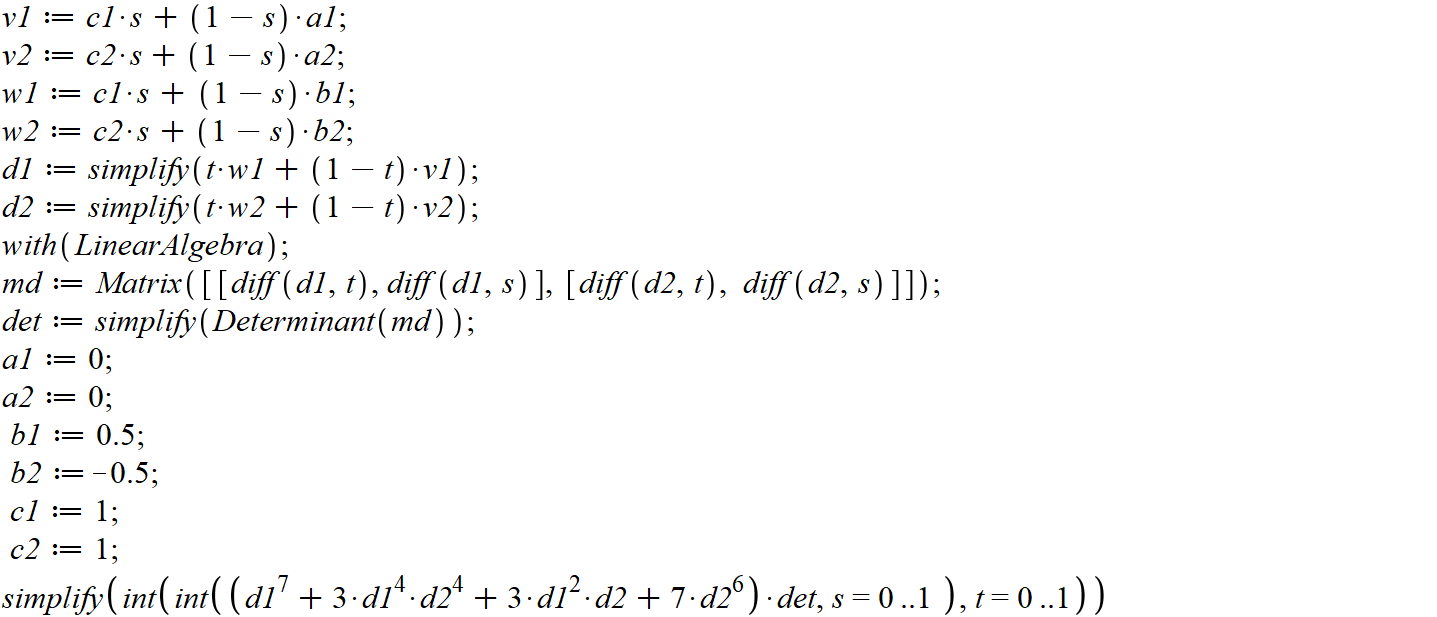
\includegraphics[width=1\textwidth]{mw_3_5_1.png}
\end{figure}


\noindent Anschließend benutzen wir die vorher implementierte Funktion \textbf{duffyInt} um das Integral numerisch zu berechnen und schätzen den Fehler ab. 

\begin{minipage}{\textwidth}
	{\color{change}
		\lstinputlisting{aufg3_5_1.m}}
\end{minipage}


\noindent Aus dem Plot des Fehlers in Abbildung \ref{fig:3_5_1} geht hervor, dass der numerische Wert des Integrals ab $n=4$ mit dem analytischen Wert (bis zur berechneten Kommastelle) überein stimmt. Das ist insofern bemerkenswert, da $f\in \SPAN\{x^iy^j:0 \leq i+j\leq 13 \} $. Jedoch ergibt sich unter der Transformation als Integrand nur ein Polynom (in $s$ und $t$) vom Grad 9, welches wie bereits vorher bemerkt mit einer 2D Quadratur vom Grad 4 exakt berechnet werden kann.

\begin{figure}[h]
	\centering
	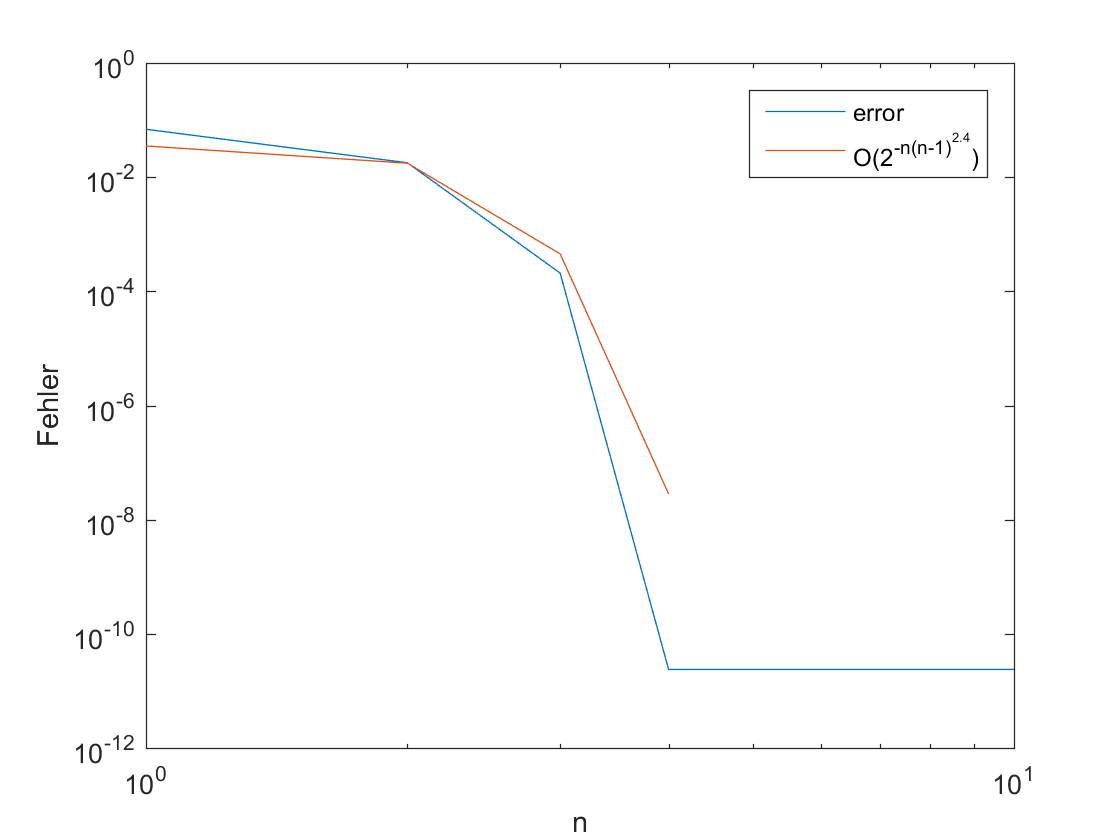
\includegraphics[width=0.8\textwidth]{plot_3_5_1.png}
	\caption{Darstellung des Fehlers der numerischen Integration von $f_1$ über $G_1$ in einem log-log Plot}
	\label{fig:3_5_1}
\end{figure}


\pagebreak
Wir betrachten als nächstes die Funktion $f_2(x,y)=\sin(50x)\sin(50y)$ auf dem Gebiet $G_2=\conv\{(1,0),(10.2),(3,4)(-1,1)\})$. Analog zu vorher berechnen wir auch hier mit Hilfe von Mapel analytisch das Integral. 

\begin{figure}[h]
	\centering
	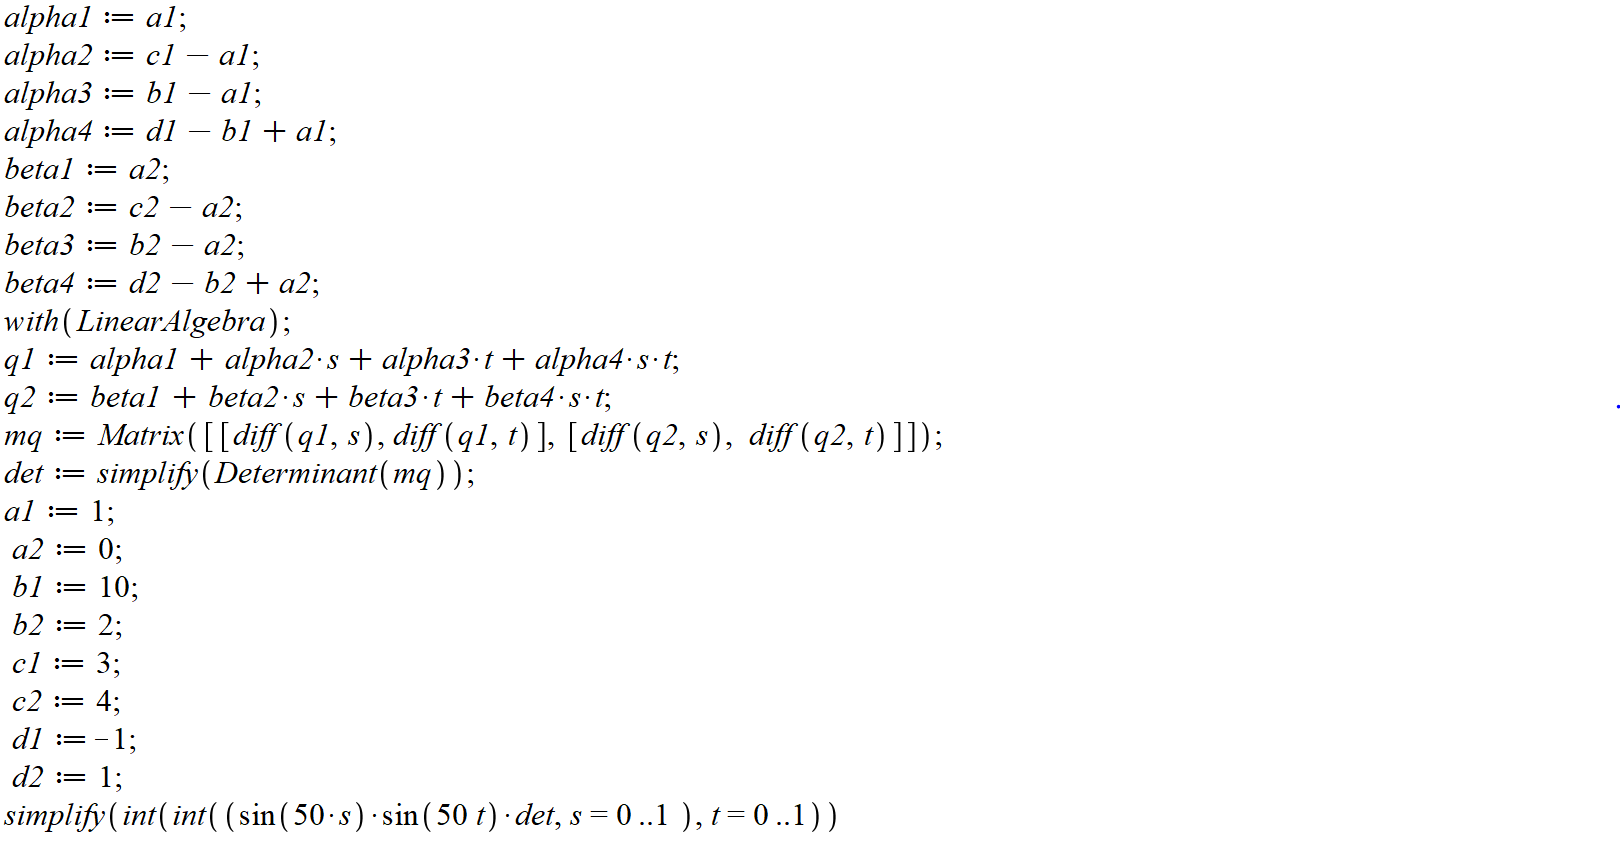
\includegraphics[width=\textwidth]{mw_3_5_2.png}
\end{figure}

\pagebreak \noindent Das Ausführen des obigen Codeausschnitts ergibt den Term $(-8/625+(37/2500)*\cos(50)+(27/125000)*\sin(50)-(27/125000)*\cos(50)*\sin(50)-(1/500)*\cos(50)^2)$ was in etwa dem Wert von 0.0003 entspricht. 


\begin{figure}[h!]
	\centering
	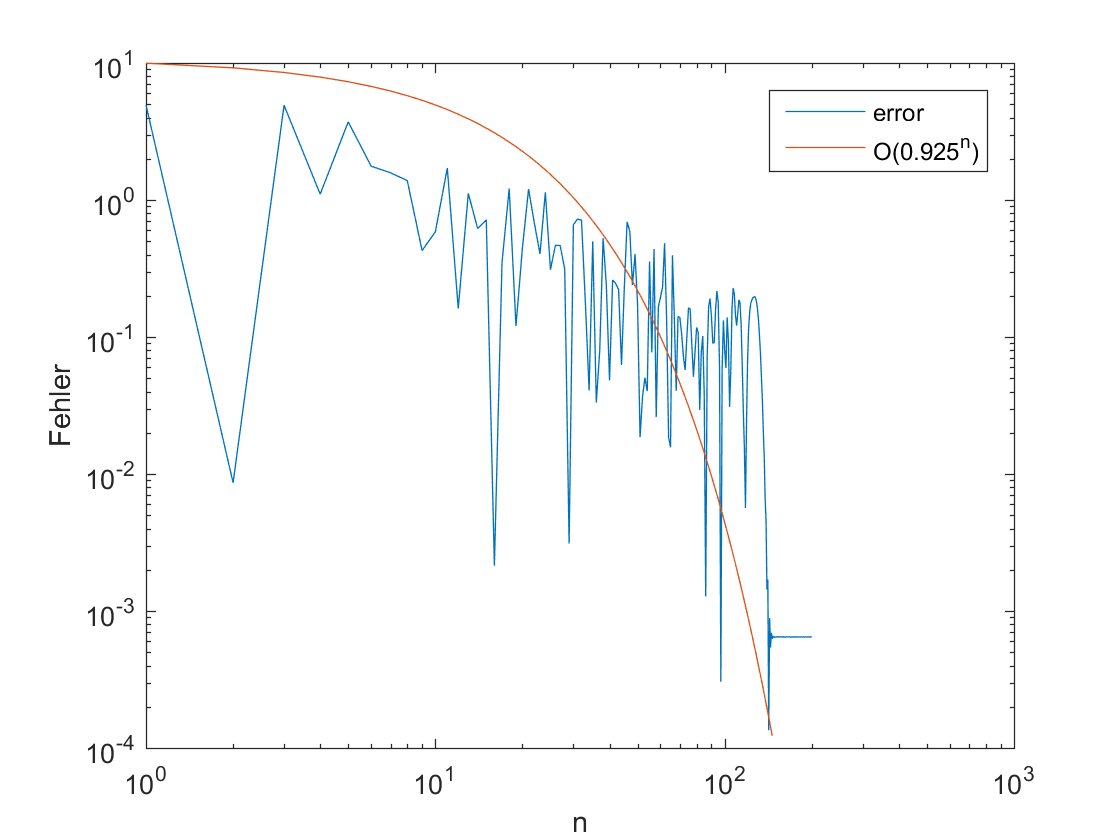
\includegraphics[width=0.8\textwidth]{plot_3_5_2.png}
	\caption{Darstellung des Fehlers der numerischen Integration von $f_2$ über $G_2$ in einem log-log Plot}
	\label{fig:3_5_2}
\end{figure}

\noindent Anschließend verwenden wir die Funktion \textbf{quadInt2}, um den numerischen Wert des Integrals zu berechnen.  Da es sich diesmal nicht um ein Polynom handelt, nähert sich der numerische Wert des Integrals zwar immer mehr dem analytischen Wert an, erreicht diesen jedoch nie. Ab einem Grad von $n=147$ entspricht der numerische Wert bis auf vier Nachkommastellen dem analytischen. Es zeigt sich weiters, dass der Trend der Konvergenz einer Funktion aus $O(0.95^n)$ ähnelt. Dieser Zusammenhang ist in Abbildung \ref{fig:3_5_2} dargestellt.


\begin{minipage}{\textwidth}	
	\color{change}
	\lstset{ 
		language=Matlab, 
		showstringspaces=false}
	\lstinputlisting{aufg3_5_2.m} 
\end{minipage}


	
	
\pagebreak
Für die Funktion $f_3(x,y)= \sqrt{\frac{9y}{(1-x^2)}}$ wissen wir bereits, dass ihr Integral über $G_3=\hat{Q}$ gegen $\pi$ konvergiert. Zur Berechnung des numerischen Integralwerts verwenden wir diesmal die Funktion \textbf{quadInt}. 

\begin{minipage}{\textwidth}	
	\color{change}
	\lstset{ 
		language=Matlab, 
		showstringspaces=false}
	\lstinputlisting{aufg3_5_3.m} 
\end{minipage}

Aus Abbildung \ref{fig:3_5_3} wird ersichtlich, dass der numerische Wert nur sehr langsam gegen den tatsächlichen konvergiert. Der Fehler verhält sich dabei etwa wie eine Funktion aus $O(n^\alpha)$ mit einem $\alpha \in (-1,-0.5)$. 
	
\begin{figure}[h]
	\centering
	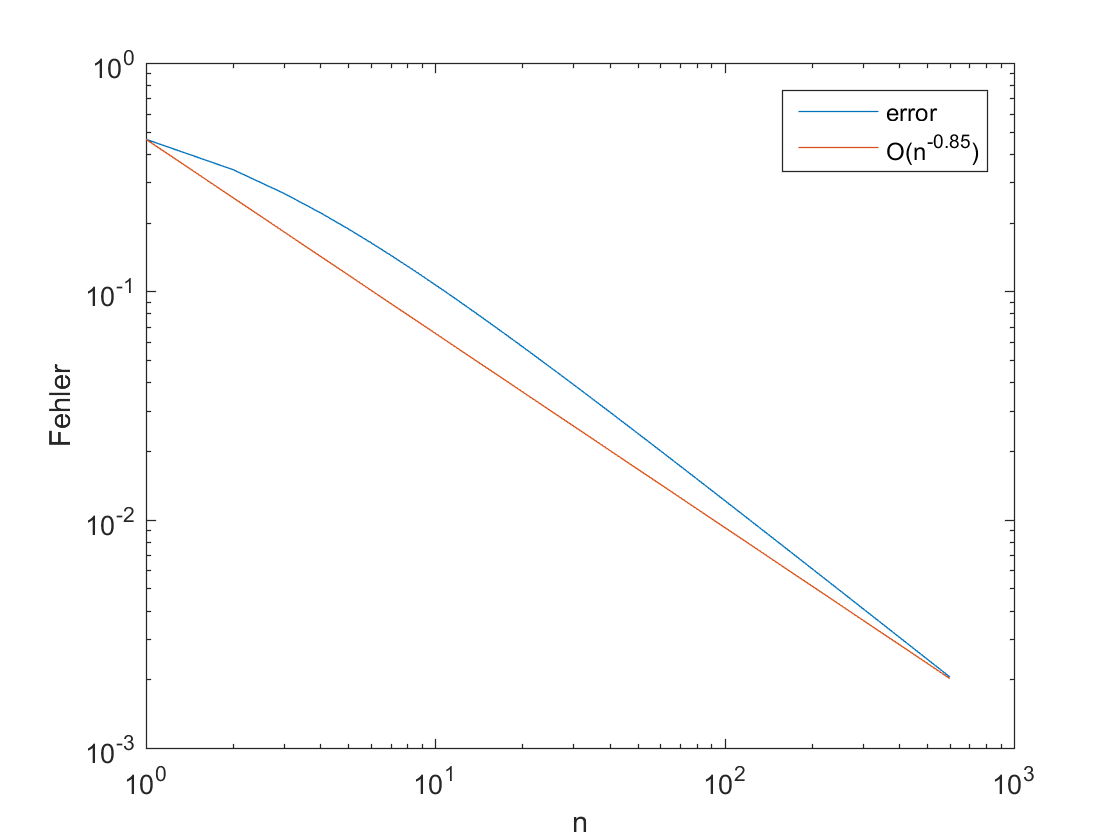
\includegraphics[width=0.8\textwidth]{plot_3_5_3.png}
	\caption{Darstellung des Fehlers der numerischen Integration von $f_3$ über $G_3$ in einem log-log Plot}
	\label{fig:3_5_3}
\end{figure}
	

\pagebreak Um die Fläche des Einheitskreises numerisch zu berechnen, approximieren wir diesen mit jeweils $2^n$ Dreiecken, benutzen eine Gaußquadratur vom Grad 0, um das Integral der  konstanten Einsfunktion über einem der Dreiecke und multiplizieren dieses Ergebnis mit $2^n$. Im folgenden wird kurz eine Möglichkeit skizziert wie man rekursiv auf die richtigen Eckpunkte eines der Dreiecke kommt.

\noindent Betrachten wir dazu folgende Skizze. Wir gehen von dem Dreieck, welches von den Punkten $a$, $b$ und $c$ aufgespannt wird aus und wollen uns den Punkt $\tilde{c} = \left(\begin{array}{ccc}
	\tilde{c_1} \\
	\tilde{c_2}\\
\end{array}\right)$ berechnen.

\vspace{14mm}
\hspace{2.7cm}
\begin{tikzpicture}
	\draw[line width=0mm,red] (0,0)--(2.3,0) node [below] {$b$};
	\draw[line width=0mm,blue] (1.2,1.2) -- (1.2,1.2) node [right=0.5cm] {$\tilde c_2$};
\draw[thick,->,blue] (-3,0)--(3,0) node[below] {$x$}; % x axis
\draw[thick,->,blue] (0,-3)--(0,3) node[left] {$y$}; % y axis

\draw[red,thick] (0,0) circle (2.5cm) node[below left] {$a$};
\draw[blue](0,0) -- (1.75,1.75) node [above right] {$\tilde{c}$};
\draw[blue](1.75,0) -- (1.75,1.75) node [below=1.75cm] {$\tilde c_1$};
\draw[red] (2.5,0) -- (0,2.5) node [above right] {$c$};
\draw[blue](1.25,1.25) -- (1.25,0)   node [below left] {$x_1$};
\draw [blue] (1.25,1.25) -- (1.25,0.75) node[below right=-0.05cm] {$x_2$};


\end{tikzpicture}\\

Durch den Satz von Pythagoras ergibt sich
\begin{equation*}
	x=(\frac{a_1+b_1}{2},\frac{a_2+b_2}{2}).
\end{equation*}  

\noindent Sei nun $\gamma$ der Winkel zwischen den Vektoren $\tilde{c}-a$ und $b-a$. Dann ist $\tilde{c_1} = \cos(\gamma)$ und $\tilde{c_2} = \sin(\gamma)$. Damit folgt
\begin{equation}
	tan \gamma = \frac{x_2}{x_1} = \frac{\sin\gamma}{\cos\gamma} = \frac{\tilde(c_2)}{\tilde(c_1)}
\end{equation}

Wir wissen aus
\begin{equation*}
	\sin(x)^2+\cos(x)^2=1, 
\end{equation*}
dass 
\begin{equation*}
	\tilde c_1^2+\tilde c_2^2=1.
\end{equation*}
Durch Lösen dieses Gleichungssystems ergibt sich 

\begin{equation*}
	\tilde c_2=\frac{c_2}{c_1+1}\sqrt{\frac{1}{(1+\frac{c_2^2}{(c_1+1)^2}}} \text{ und } \tilde c_1 = \sqrt{\frac{1}{(1+\frac{c_2^2}{(c_1+1)^2}}}.
\end{equation*}

\noindent Dieses Verfahren wird nun iterativ angewandt um beliebig kleine Dreiecke zu bekommen. Nun kann die Funktion \textbf{duffyInt} verwendet werden, um die Fläche des Einheitskreises zu approximieren. 

\begin{minipage}{\textwidth}	
	\color{change}
	\lstset{ 
		language=Matlab, 
		showstringspaces=false}
	\lstinputlisting{aufg3_5_4.m} 
\end{minipage}

Aus Abbildung \ref{fig:3_5_4} wird ersichtlich, dass dieses Verfahren $\pi$ zu berechnen wesentlich schneller zum Ziel führt. Der Fehler entwickelt sich mit steigender Anzahl der Ecken wie eine Funktion aus $O(n^{-2})$ ein weitere Vorteil dieser Variante ist, dass nur Polynome nullten Grades berechnet werden müssen. 

\begin{figure}[h]
	\centering
	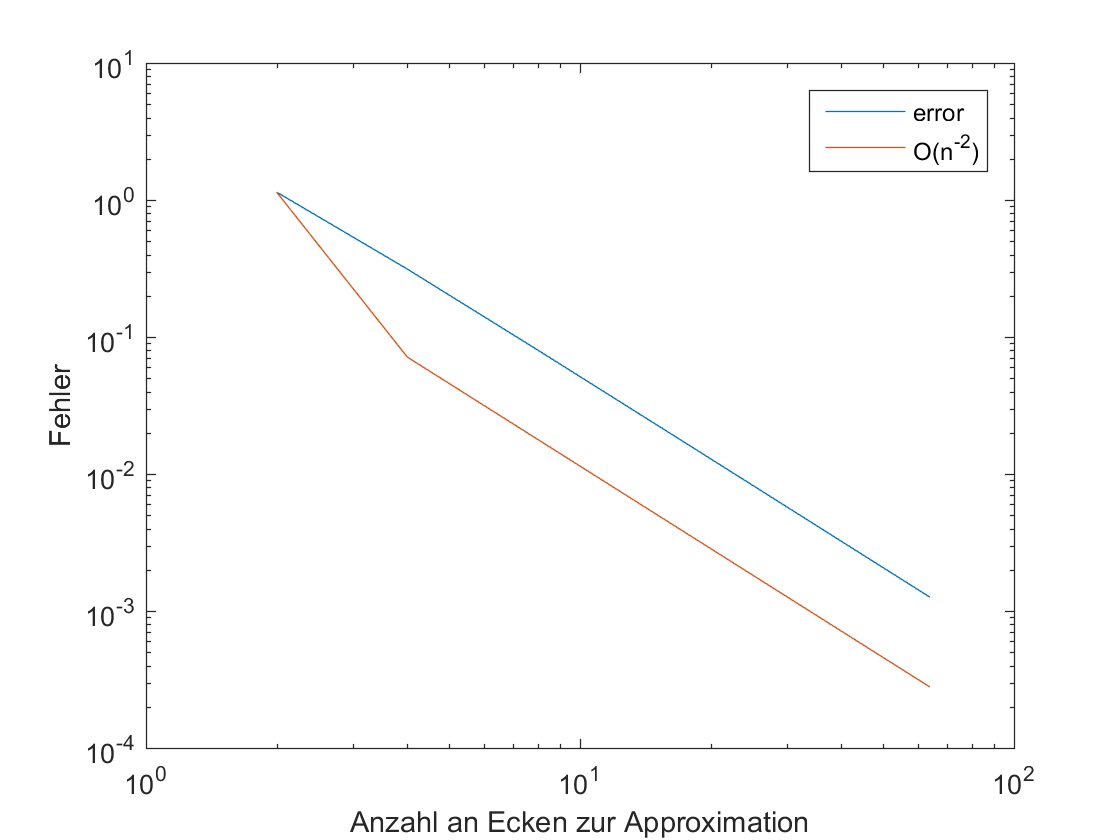
\includegraphics[width=0.8\textwidth]{plot_3_5_4.png}
	\caption{Darstellung des Fehlers der numerischen Berechnung der Fläche des Einheitskreises über Approximation mittels Dreiecken}
	\label{fig:3_5_4}
\end{figure}



					
				
				
		
		
	
			
	
	
		
	
			
	
	


\end{document}